\section{Auswertung}
\label{sec:Auswertung}
\subsection{Anlaufverhalten}
In diesem Szenario wird der Pitchwinkel schrittweise variiert, und für jede Servo-Einstellung  wird das abgelesene Moment aufgezeichnet. Anschließend wird der Pitchwinkel sowohl durch Kalibrierung als auch unter Verwendung des Momentenbeiwerts berechnet.
\begin{table}[ht!]
    \centering
    \caption{Messwerte}
    \label{tab_Messwerte_Anlauf_230615}
    \begin{tabular}{|l|l|l|l|l|l|}
        \hline
        \rowcolor[HTML]{70AD47} 
        {\color[HTML]{FFFFFF} \textbf{$v_{Wind,Soll}$}} & {\color[HTML]{FFFFFF} \textbf{$v_{Wind,ist}$}} & {\color[HTML]{FFFFFF} \textbf{Pitch abgelesen}} & {\color[HTML]{FFFFFF} \textbf{Pitch erwartet}} & {\color[HTML]{FFFFFF} \textbf{$c_{M,0}$}} & {\color[HTML]{FFFFFF} \textbf{$c_{M,1}$}} \\ \hline
        \rowcolor[HTML]{70AD47} 
        in m/s                                         & in m/s                                      & in °                                            & in °                                           & -                                      & -                                      \\ \hline
        \rowcolor[HTML]{E2EFDA} 
        1                                              & 1                                           & -                                               & -                                              & 0,666                                  & 0,666                                  \\ \hline
        \rowcolor[HTML]{C6E0B4} 
        1,5                                            & 1,6                                         & 45                                              & 44,98                                              & 0,296                                  & 0,260                                  \\ \hline
        \rowcolor[HTML]{E2EFDA} 
        2                                              & 2,1                                         & 32                                              & 34,15                                              & 0,167                                  & 0,151                                  \\ \hline
        \rowcolor[HTML]{C6E0B4} 
        2,5                                            & 2,45                                        & -5                                              & -3,51                                       & 0,107                                  & 0,111                                  \\ \hline
    \end{tabular}
\end{table}

In \autoref{fig:Pitch_Wind} ist die Kalibrierungsunschärfe dargestellt. Der kalibrierte Wert weicht vom Einstellwert ab.
\begin{figure}[H]
    \centering
    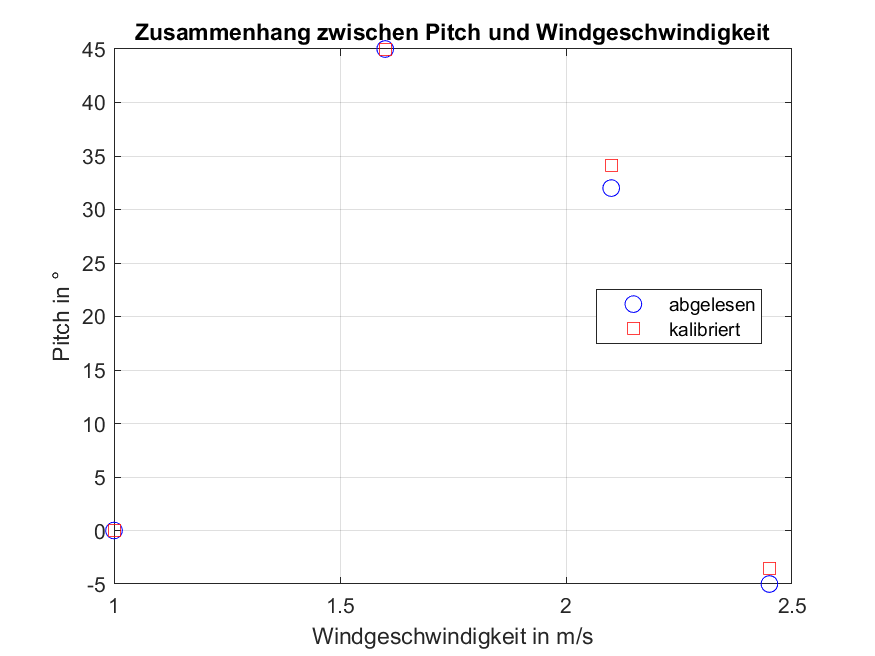
\includegraphics[width=0.9\textwidth]{plot1}
    \caption{Zusammenhang zwischen Pitch und Windgeschwindigkeit}
    \label{fig:Pitch_Wind}
\end{figure}

In \autoref{fig:Momentenbeiwert_Anlauf} sind der theoretische Momentenbeiwert $c_{M,0}$ und der praktische $c_{M,1}$ in Abhängigkeit der Windgeschwindigkeit dargestellt.
Das praktische Anlaufmoment ist gegenüber dem theoretischen etwas niedriger, was vor allem durch die Abweichung der Windgeschwindigkeit vom Soll-Wert zu erklären ist.
\begin{figure}[H]
    \centering
    \includegraphics[width=0.9\textwidth]{cm_Anlauf}
    \caption{Momentenbeiwert $c_M$ im Anlauf}
    \label{fig:Momentenbeiwert_Anlauf}
\end{figure}

\subsection{Leerlauf und maximale Schnelllaufzahl}
Im Rahmen der Untersuchungen wurden bei verschiedenen konstanten Windgeschwindigkeiten verschiedene Messungen durchgeführt.
 Die Auswertung dieser Messungen beinhaltet mehrere wichtige Parameter, die für jede der untersuchten Windgeschwindigkeiten dargestellt werden. Die entsprechenden Werte sind in der folgenden Tabelle zusammengefasst:

\begin{table}[H]
    \centering
    \caption{Messwerte Leerlaufverhalten und maximale Schnelllaufzahl}
    \label{tab_Messwerte_Leerlaufverhalten}
    \begin{tabular}{|l|l|l|l|l|l|}
    \hline
    \rowcolor[HTML]{70AD47} 
    {\color[HTML]{FFFFFF} \textbf{Pitch}} & {\color[HTML]{FFFFFF} \textbf{Pitch2}} & {\color[HTML]{FFFFFF} \textbf{$U_{Gen}$}} & {\color[HTML]{FFFFFF} \textbf{n}} & {\color[HTML]{FFFFFF} \textbf{$u_{tip}$}} & {\color[HTML]{FFFFFF} \textbf{$\lambda$}} \\ \hline
    \rowcolor[HTML]{70AD47} 
    soll                                  & berechnet                              & abgelesen                                          & abgelesen                                & berechnet                                            & berechnet                                      \\ \hline
    \rowcolor[HTML]{70AD47} 
    in °                                  & in °                                   & in V                                               & in min-1                                 & in m/s                                               & -                                              \\ \hline
    \rowcolor[HTML]{C6E0B4} 
    -5                                    & -3,51                                  & 8,2                                                & 2068,7                                   & 36,83                                          & 5,67                                    \\ \hline
    \rowcolor[HTML]{E2EFDA} 
    0                                     & -1,34                                  & 9                                                  & 2272                                     & 40,45                                          & 6,22                                    \\ \hline
    \rowcolor[HTML]{C6E0B4} 
    5                                     & 5,45                                   & 9,48                                               & 2390,9                                   & 42,56                                          & 6,55                                    \\ \hline
    \rowcolor[HTML]{E2EFDA} 
    10                                    & 12,17                                  & 9,9                                                & 2512,5                                   & 44,73                                          & 6,88                                    \\ \hline
    \rowcolor[HTML]{C6E0B4} 
    15                                    & 18,01                                  & 9,78                                               & 2476,1                                   & 44,08                                          & \cellcolor[HTML]{FFC000}6,78                                    \\ \hline
    \rowcolor[HTML]{E2EFDA} 
    20                                    & 23,24                                  & 9,2                                                & 2344,8                                   & 41,74                                          & 6,42                                     \\ \hline
    \rowcolor[HTML]{C6E0B4} 
    25                                    & 28,22                                  & 8,6                                                & 2187,5                                   & 38,94                                          & 5,99                                    \\ \hline
    \rowcolor[HTML]{E2EFDA} 
    30                                    & 32,81                                  & 8                                                  & 2022,2                                   & 36,00                                           & 5,54                                     \\ \hline
    \rowcolor[HTML]{C6E0B4} 
    35                                    & 37,10                                 & 7,3                                                & 1863,1                                   & 33,17                                          & 5,10                                    \\ \hline
    \rowcolor[HTML]{E2EFDA} 
    40                                    & 40,97                                  & 6,85                                               & 1739,5                                   & 30,97                                          & 4,76                                    \\ \hline
    \rowcolor[HTML]{C6E0B4} 
    45                                    & 44,98                                  & 6,6                                                & 1670,8                                   & 29,74                                         & 4,58                                    \\ \hline
    \rowcolor[HTML]{E2EFDA} 
    50                                    & 48,87                                  & 6,2                                                & 1573,1                                   & 28,00                                         & 4,31                                    \\ \hline
    \end{tabular}
    \end{table}
\newpage
     Dabei wurden die Pitch-Einstellung bzw. der rechnerisch korrigierte Pitch-Winkel, um die Neigung der Rotorblätter und deren 
     präzise Ausrichtung zur Anströmung des Windes zu ermitteln, in der Tabelle dargestellt. Ebenfalls wurde die Generator-Leerlaufspannung $U_{Gen_0}$ erfasst, 
     um die elektrischen Eigenschaften des Generators im Leerlauf zu untersuchen. Ein weiterer relevanter Wert ist die Leerlaufdrehzahl des Rotors $n_0$, 
     die Auskunft über die Rotor-Drehzahl bei fehlender Last gibt. Zudem wurde die Blattspitzengeschwindigkeit des Rotors $u_{tip}$ ermittelt, um die Geschwindigkeit an den äußersten Enden der Rotorblätter zu bestimmen. 
     Die Schnelllaufzahl $\lambda$, als Verhältnis zwischen der relativen Windgeschwindigkeit und der Blattspitzengeschwindigkeit, wurde untersucht, um die aerodynamische Effizienz des Systems zu bewerten. Besonders wichtig war das Vermerken der maximalen
    Schnelllaufzahl $\lambda_{max}$ für jede Windgeschwindigkeit $v_{Wind}$, um die optimale Auslastung des Rotors bei verschiedenen Windbedingungen zu erkennen. Die Auswertung dieser Parameter lieferte
    wertvolle Erkenntnisse über das Verhalten des Windkraftsystems bei unterschiedlichen Windgeschwindigkeiten und ermöglichte die gezielte Verbesserung der Leistungsfähigkeit und Effizienz der Anlage. Diese Erkenntnisse tragen zur Weiterentwicklung und 
    Optimierung von Windenergieanlagen bei,
     um einen effizienten und nachhaltigen 
     Beitrag zur Energieerzeugung aus erneuerbaren Quellen zu gewährleisten.

\begin{equation}
    \centering
    u = 2 \pi \cdot r_{Rotor} \cdot \frac{n}{60 \frac{s}{min}}
    \label{eq:230615_Umfangsgeschwindigkeit}
\end{equation}

$$    u = 2 \pi \cdot 0,17m \cdot \frac{2512,5 \frac{1}{min}}{60 \frac{s}{min}}\approx 44,73\frac{m}{s} $$

\begin{equation}
    \centering
    \lambda = \frac{u}{v_1}
    \label{eq:230615_Schnelllaufzahl}
\end{equation}

$$\lambda = \frac{44,73}{6,5 \frac{m}{s}}\approx 6,88$$

Erklärung Graphen, alle Kurvenverläufe ähneln sich und nehmen ihr Maximum bei der optimalen Schnelllaufzahl an.
\begin{figure}[H]
    \centering
        \begin{minipage}[t]{0.4\textwidth}
            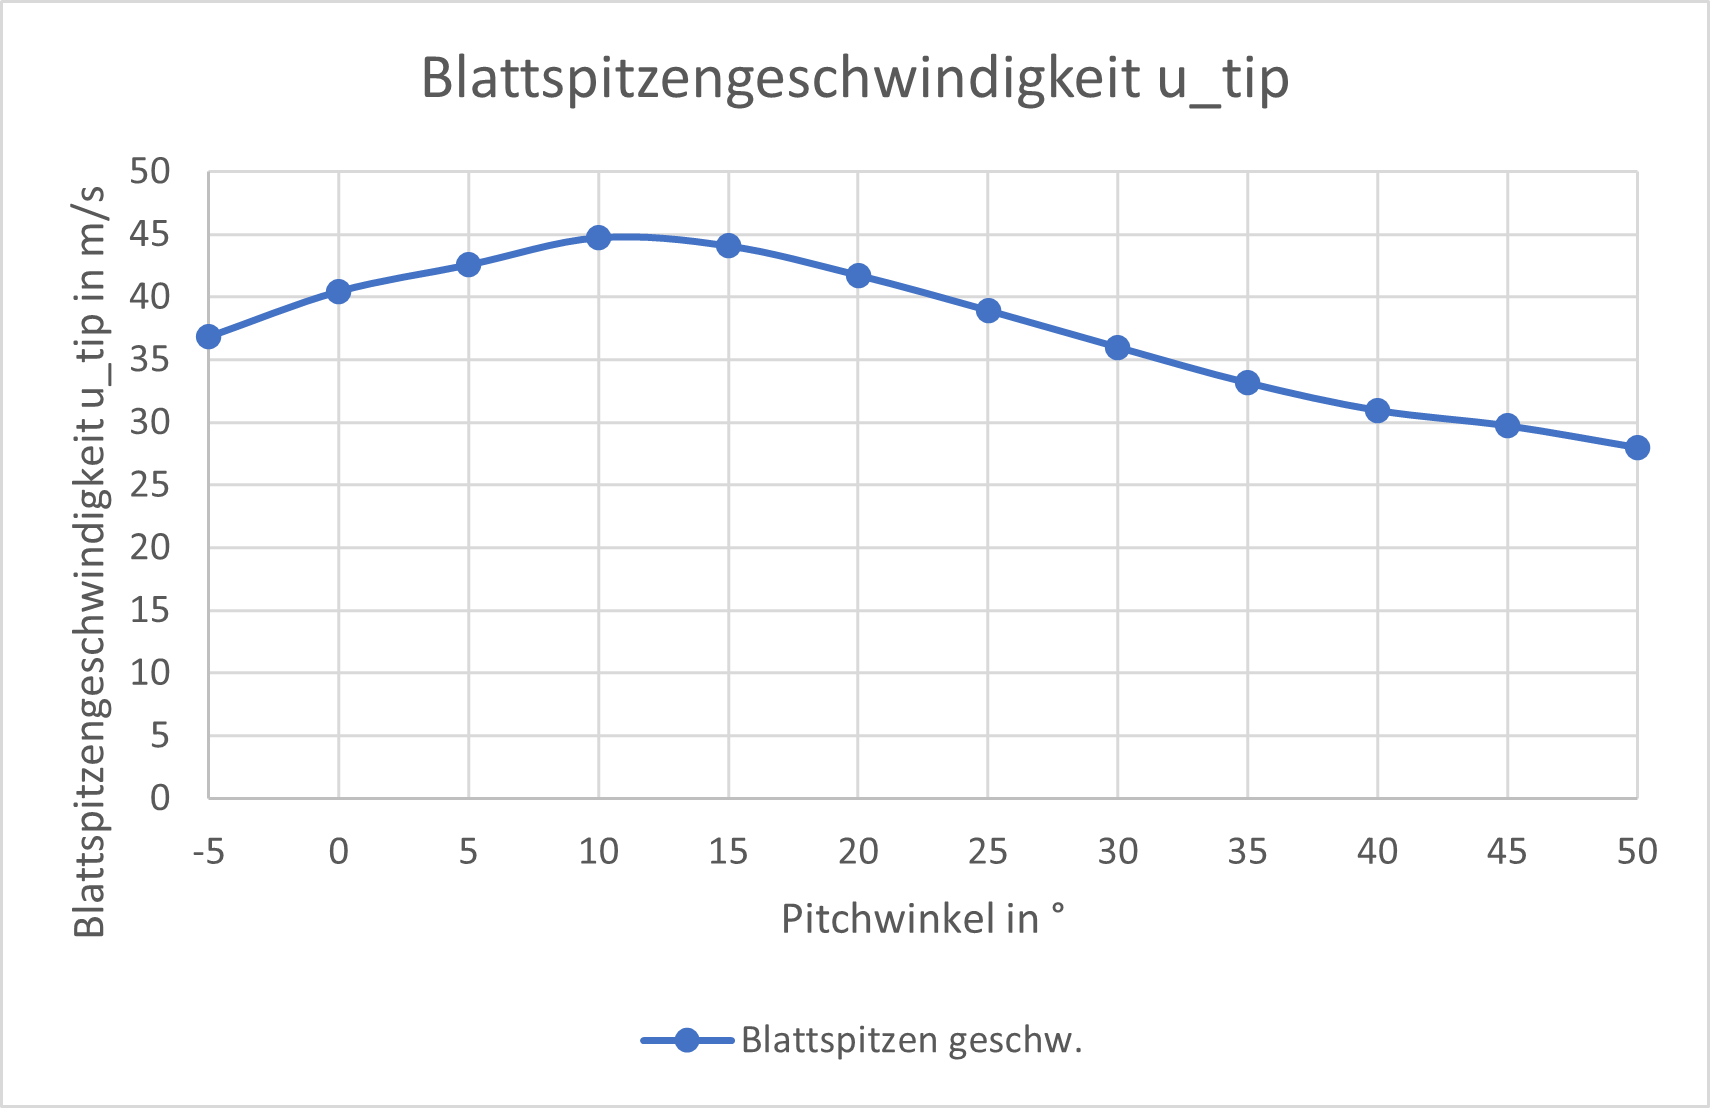
\includegraphics[width=\textwidth]{utip}
            \caption{Blattspitzengeschwindigkeit $U_{tip}$}
            \label{fig:utip}
        \end{minipage}
        \begin{minipage}[t]{0.4\textwidth}
            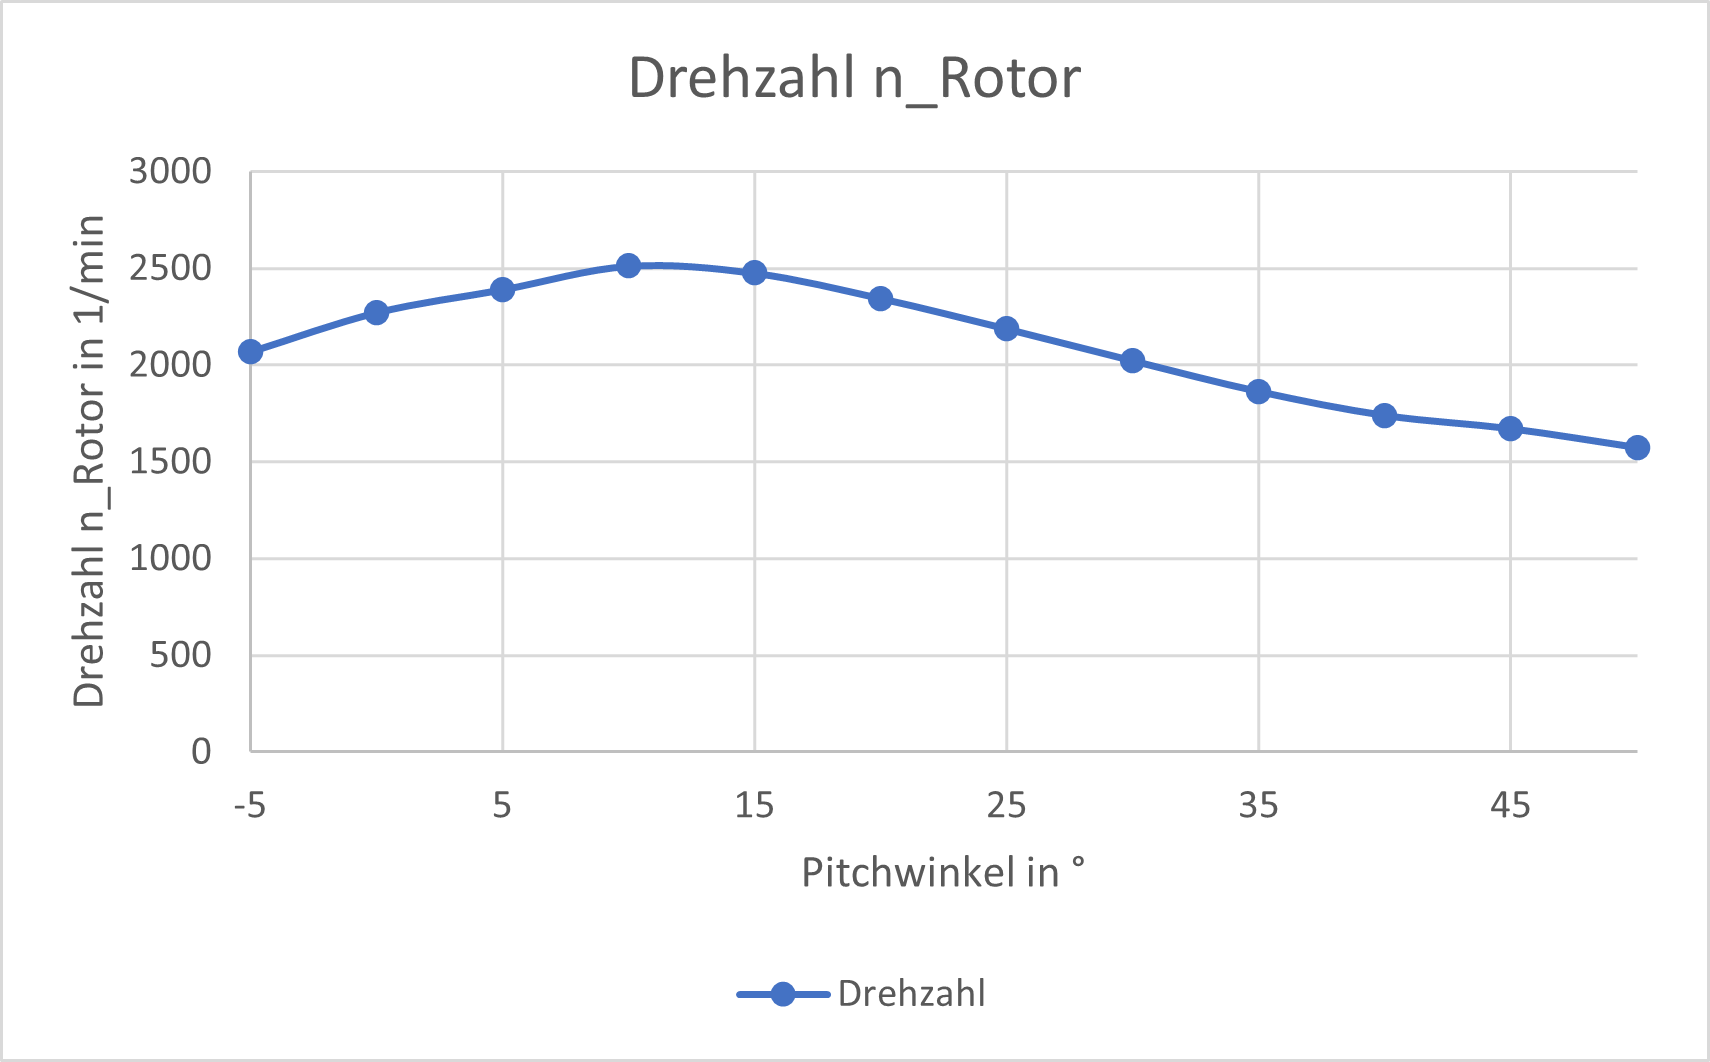
\includegraphics[width=\textwidth]{Drehzahl}
            \caption{Drehzahl $n_{Rotor}$}
            \label{fig:n_rotor}
        \end{minipage}
        \begin{minipage}[b]{0.4\textwidth}
            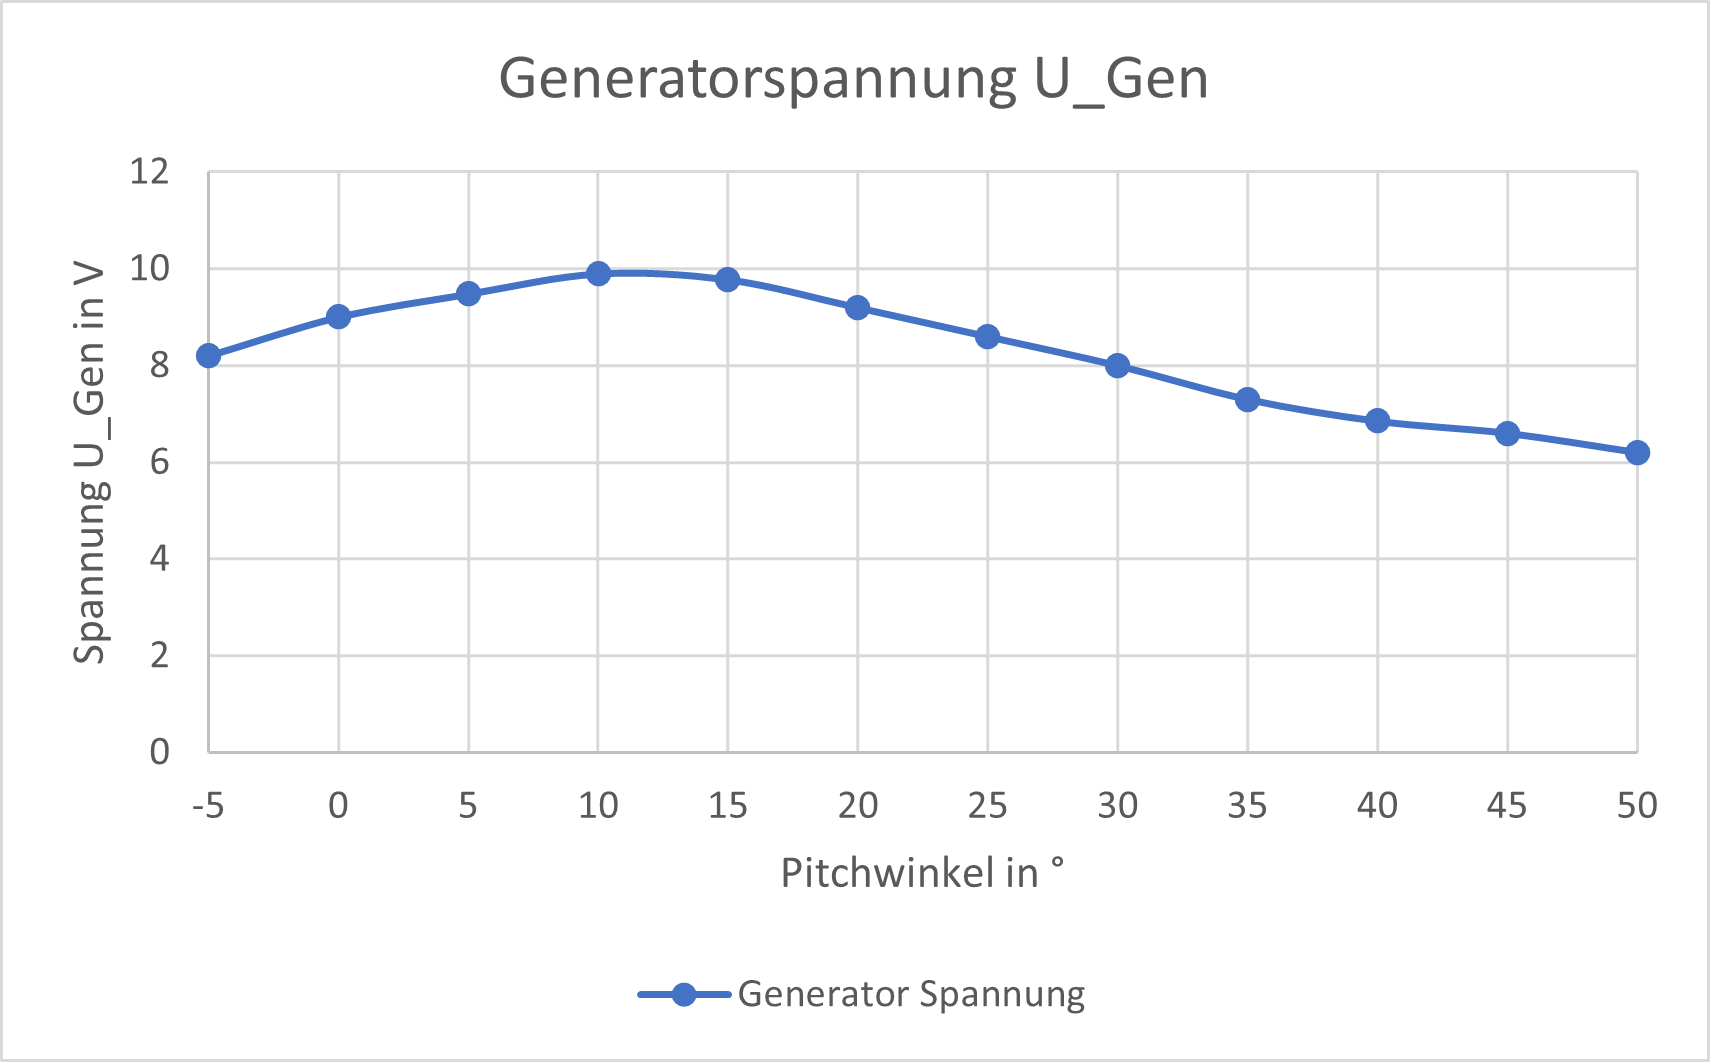
\includegraphics[width=\textwidth]{UGen}
            \caption{Generatorspannung $U_{Gen}$}
            \label{fig:UGen}
        \end{minipage}
        \begin{minipage}[b]{0.4\textwidth}
            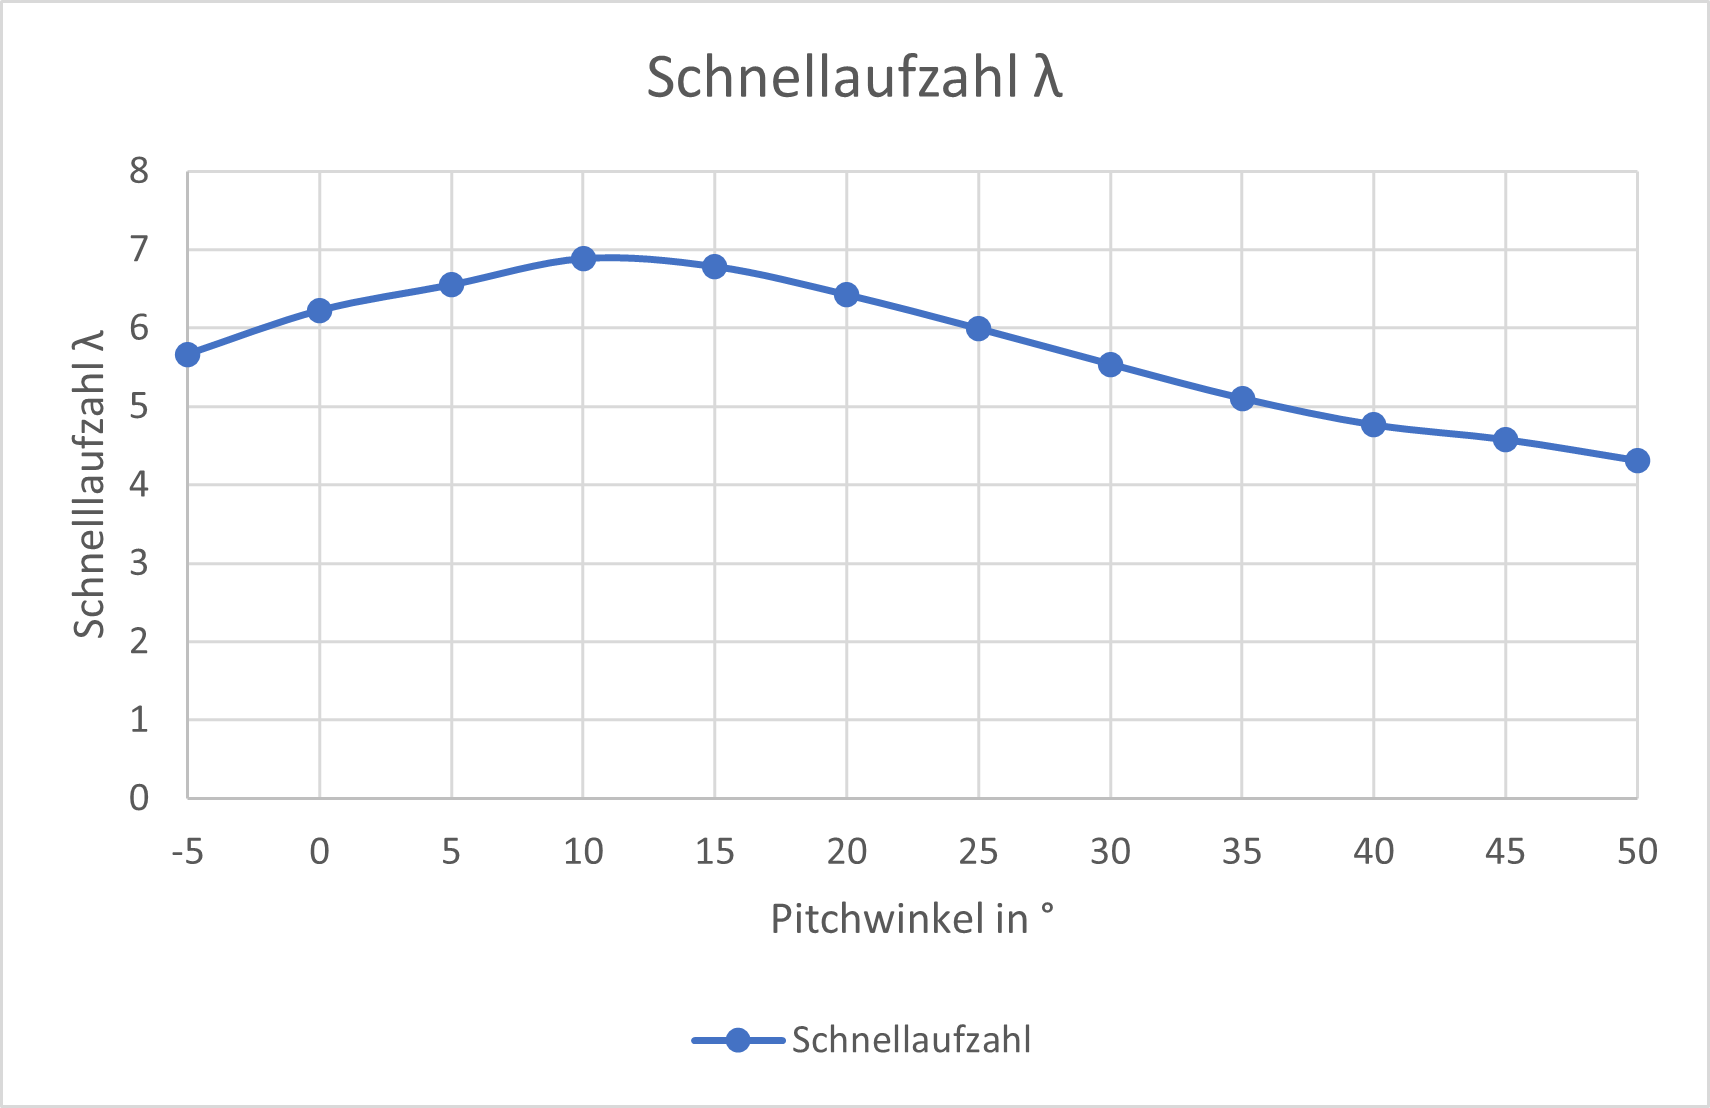
\includegraphics[width=\textwidth]{schnelllaufzahl}
            \caption{Schnelllaufzahl $\lambda$}
            \label{fig:lambda}
        \end{minipage}
    \end{figure}  

\subsection{Dimensionslose Kennzahlen}
Das folgende Kapitel widmet sich den ermittelten dimensionslosen Kennzahlen.
Für alle berechneten Werte wird eine Beispielrechnung angegeben und eine Einordnung vorgenommen.
Die gemessenen und ermittelten Werte sind in \autoref{tab:2307028_DimensionsloseKennzahlen} vollständig einzusehen.
\subsubsection*{Turbulenzintensität der gemessenen Windgeschwindigkeit}
\begin{figure}[H]
    \centering
    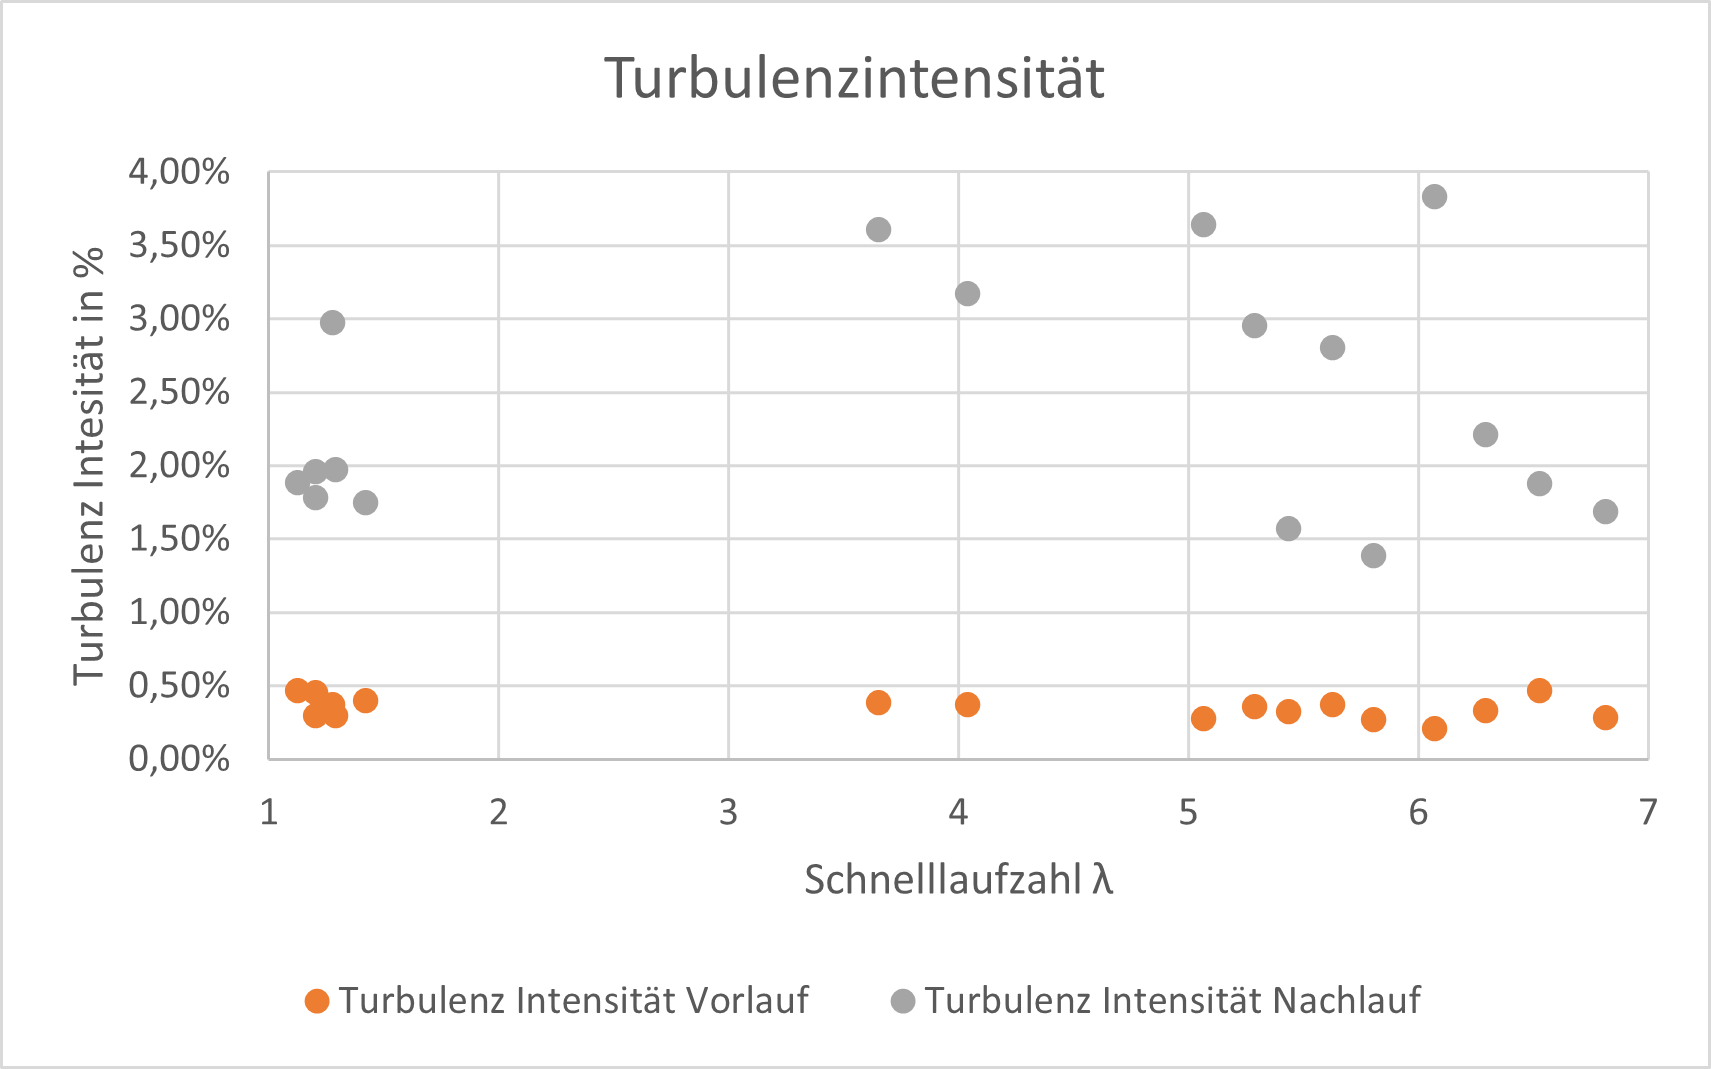
\includegraphics[width=0.8\textwidth]{turbint}
    \caption{Turbulenzintensität Vorlauf und Rücklauf}
    \label{fig:Turbulenzintensität}
\end{figure}
Die Turbulenzintensität ist im Vorlauf mit Werten bis 0,5\% verschwindend gering und damit vernachlässigbar. Die Turbulenzintensität des Nachlaufs unterliegt starken Schwankung, was auf die Versuchsbedingungen zurückzuführen ist.

\subsubsection*{Geschwindigkeitsreduktion$\frac{v_3}{v_1}$}
Unter Lastzunahme nimmt die Geschwindigkeitsreduktion bis zur Auslegungsschnelllaufzahl ab, anschließend steigt das Verzögerungsverhältnis wieder. 
\begin{figure}[H]
    \centering
    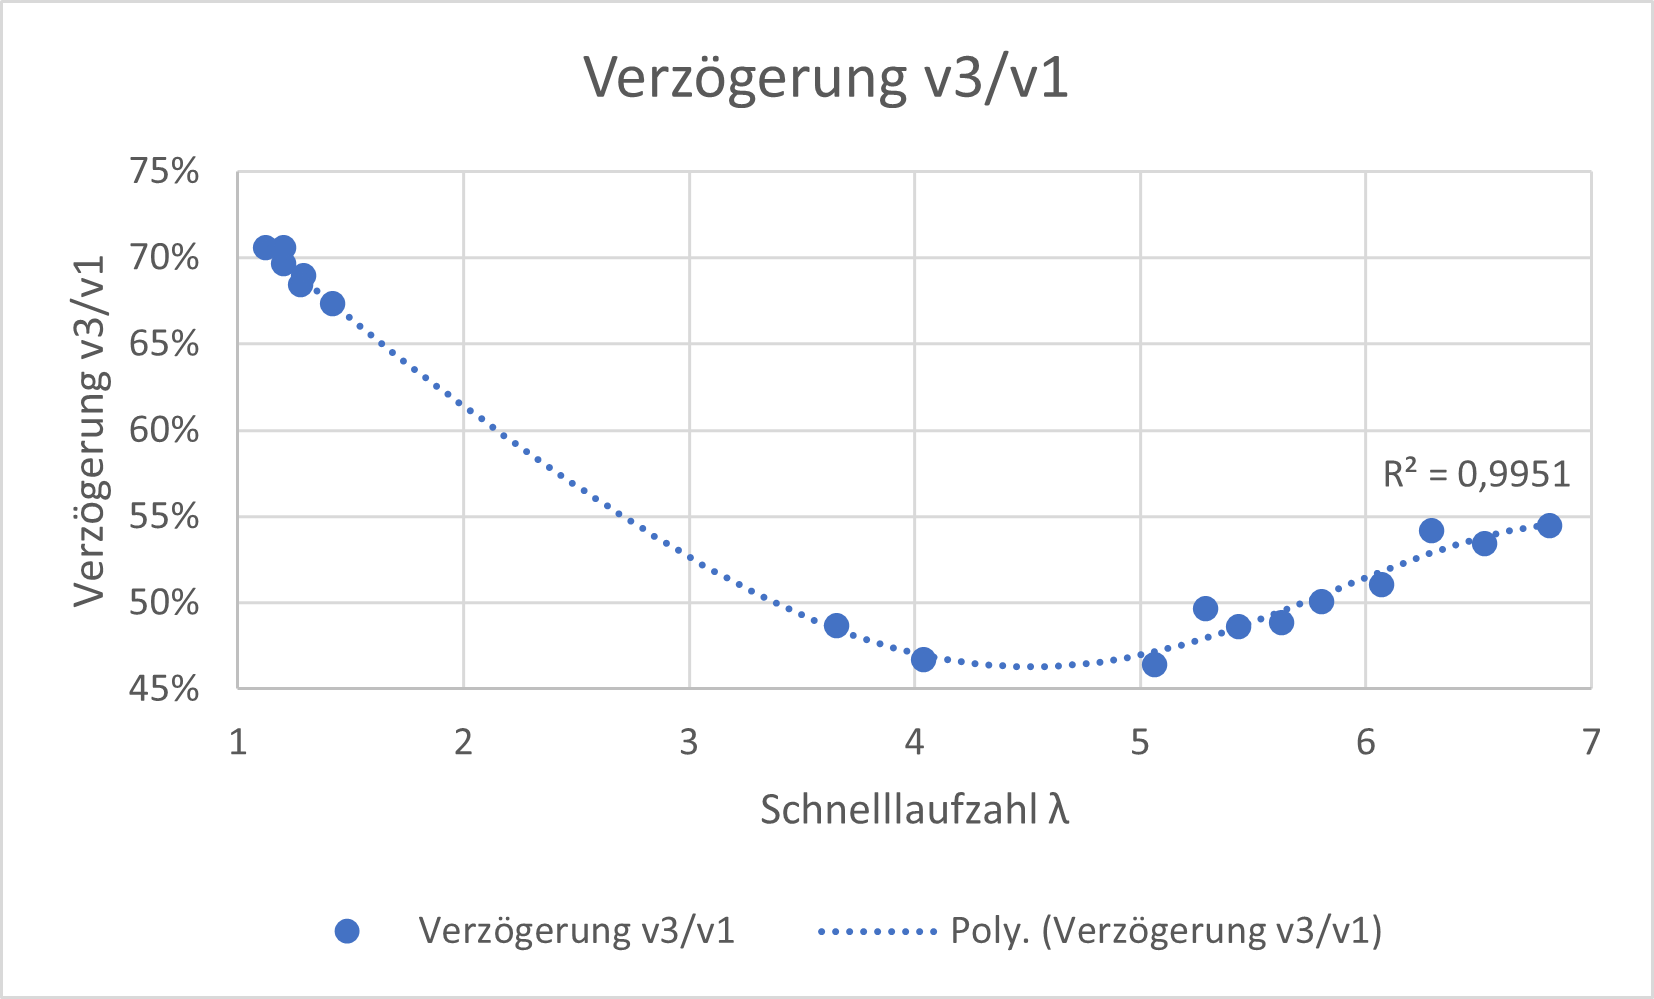
\includegraphics[width=0.8\textwidth]{v3_v1}
    \caption{Geschwindigkeitsreduktion $\frac{v3}{v1}$}
    \label{fig:Geschwindigkeitsreduktion}
\end{figure}

\subsubsection*{Windleistung $P_{Wind}$}
Zu Begin wird die reine theoretische Windleistung über Formel \autoref{eq:230615_Leistung_Wind} ermittelt:

\begin{equation}
    \centering
    P_{Wind} = \frac{\rho}{2} \cdot \pi \cdot r_{Rotor}^2 \cdot v_1^3
    \label{eq:230615_Leistung_Wind}
\end{equation}

Es werden hierfür die gemessenen und gegebenen Kenndaten eingefügt:
$$P_{Wind} = \frac{1,2 \frac{kg}{m^3}}{2} \cdot \pi \cdot (0,17 m)^2 \cdot (6,43)^3 \approx 14,46 W$$
Die theoretische Leistung, die aus dem Wind entnommen werden kann, liegt bei 14,46W.

\subsubsection*{Rotordrehzahl $n_{Rotor}$}
Über die Lastregelung ist eine variable Drehzahlregelung möglich. In \autoref{tab:2307028_DimensionsloseKennzahlen} ist die Regelung anhand der Werte erkennbar. Eine Erhöhung der Last führt zu einem Absinken der Drehzahl.
\subsubsection*{Drehmoment $M_{Gen}$}
Ausgehend von der Annahme,
dass entgegen der Beschriftung in der LabView-Tabelle das Generatordrehmoment in mV gemessen wird und einer Umrechnung bedarf, 
werden unter Verwendung von \autoref{eq:230615_Genratormoment} die benötigten Werte ermittelt:

\begin{equation}
    \centering
    M_{Gen} = 33,931\frac{mNm}{mV} \cdot U_{Rotor} + 3,1519 mNm - M_{Reibung}
    \label{eq:230615_Genratormoment}
\end{equation}

Eine exemplarische Rechnung mit gemessenen Werte für das Generatormoment $M_{Gen}$:

$$M_{Gen} = 33,931\frac{mNm}{mV} \cdot 2,1631 + 3,1519 mNm - 6,3mNm \approx 70,25 mNm$$
Das Nenndrehmoment des Generators liegt bei $71 mNm$. Für die exemplarische Betrachtung und für den Vergleich mit Tabellenwerten werden die Werte aus der betreffenden Messreihe verwendet.
\subsubsection*{Mechanische Leistung $P_{Mech}$}
Ausgehend vom neu berechneten Generatormoment ist die mechanische Leistung über \autoref{eq:230615_Mechanischeleistung} bestimmbar:
\begin{equation}
    \centering
    P_{Mech} = M_{Gen} \cdot 2 \pi \frac{n}{60\frac{s}{min}}
    \label{eq:230615_Mechanischeleistung}
\end{equation}
Für den im vorherigen Schritt berechneten Wert beträgt die mechanische Leistung: 
$$P_{Mech} = 70,25mNm \cdot 2 \pi \frac{1318,4 \frac{1}{min}}{60\frac{s}{min}} \approx 9,7W$$

\subsubsection*{Momentenbeiwert $c_m$}
Der Momentenbeiwert wird über \autoref{eq:230615_Momentenbeiwert} ermittelt:
\begin{equation}
    \centering
    c_M = \frac{M_{Gen}}{ \frac{\rho}{2} \cdot \pi \cdot r_{Rotor}^3 \cdot v_1^2}
    \label{eq:230615_Momentenbeiwert}
\end{equation}
Für das exemplarische Generatormoment von $M_{Gen} = 70,25mNm$ beträgt der Momentenbeiwert:
$$c_M = \frac{70,25mNm}{ \frac{1,2 \frac{kg}{m^3}}{2} \cdot \pi \cdot (0,17 m)^3 \cdot (6,43)^2}\approx 0,184$$

\begin{figure}[H]
    \centering
    \includegraphics[width=0.6\textwidth]{cm_diagramm}
    \caption{Momentenbeiwert $c_M$ in Abhängigkeit von Schnelllaufzahl $\lambda$}
    \label{fig:Momentenbeiwert}
\end{figure}

\subsubsection*{Generatorleistung $P_{el}$}
Die Generatorleistung $P_{el}$ wird über \autoref{eq:230615_Elektrische_Leistung} berechnet:
\begin{equation}
    \centering
    P_{El} = U \cdot I
    \label{eq:230615_Elektrische_Leistung}
\end{equation}

Für die verwendete Messreihe beträgt die elektrische Leistung:
$$P_{El} = 3V \cdot 0,915A \approx 2,745W$$


\subsubsection*{Leistungsbeiwert $c_p$}
\autoref{eq:230615_Leistungsbeiwert} gibt die Berechnung des Leistungsbeiwerts an:
 \begin{equation}
     \centering
     c_P = c_M \cdot \lambda
     \label{eq:230615_Leistungsbeiwert}
 \end{equation}
Exemplarisch beträgt der $c_P$ mit den ermittelten Werten $c_M = $ und $\lambda =$:
 $$c_P = c_M \cdot \lambda$$

 Der Leistungsbeiwert übersteigt den theoretischen Leistungsbeiwert von Betz. Ein Wert von 67\% ist nicht realistisch. Ein erwartbarer Wert für eine Windkraftanlage in der Labordimensionierung liegt bei $\approx 0,3$. Der ermittelte Wert ist somit um den Faktor zwei größer als der zu erwartende Wert. Zurückzuführen ist diese Beobachtung entweder auf einen Messfehler oder einen Berechnungsfehler, während der Auswertung. Durch mehrmalige Prüfung konnte die Fehlerquelle nicht lokalisiert werden. Eine Vermutung ist, die getroffene Annahme für die Umrechnung vom Drehmoment ist fehlerhaft.
 \begin{figure}[H]
    \centering
    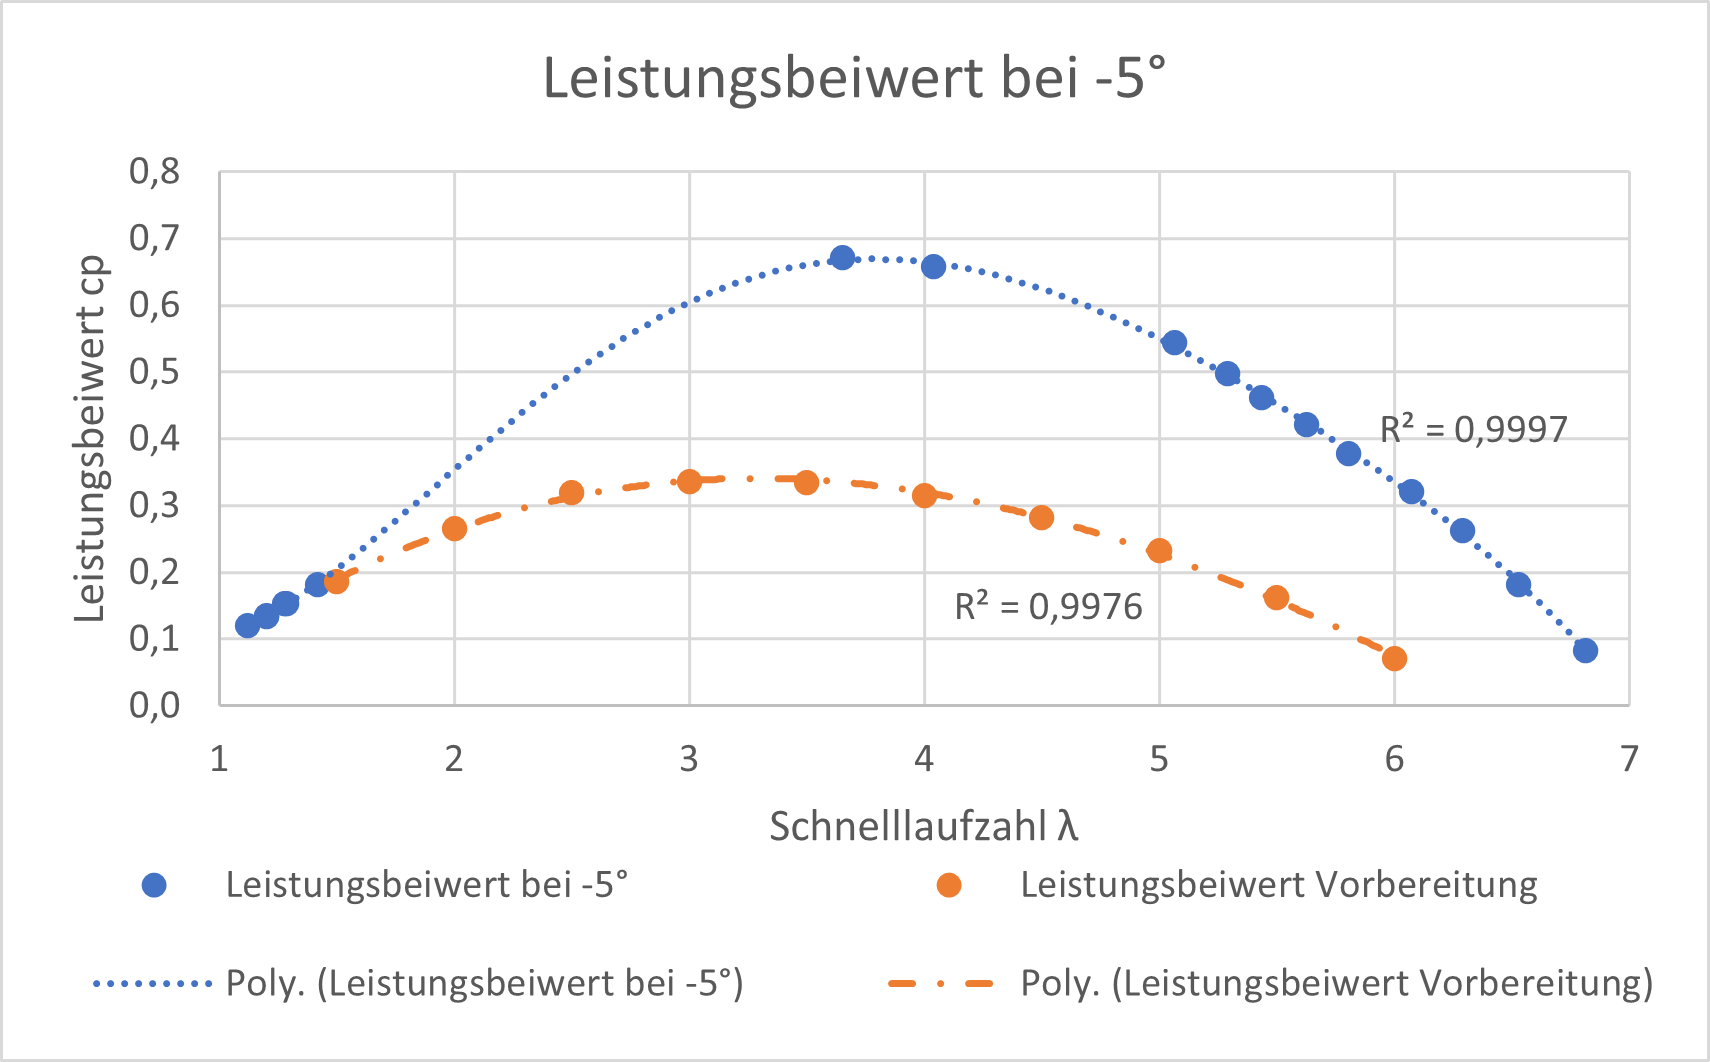
\includegraphics[width=0.9\textwidth]{cp_Last}
    \caption{Leistungsbeiwert $c_P$ in Abhängigkeit von Schnelllaufzahl $\lambda$}
    \label{fig:cp_last}
\end{figure}
\subsubsection*{Generatorspannung $U_{Gen}$}
Mit zunehmender Last sinkt die Generatorspannung $U_{Gen}$, weil der Generator
mehr erzeugt als vorher, dadurch die Drehzahl des Generators erhöht, die Verluste
steigen und dadurch endgültig die Spannung sinkt. 
\subsubsection*{Generatorstrom $I_{Gen}$}
Mit zunehmender Last steigt der Generatorstrom I, weil die Drehzahl erhöht
wird und somit mehr Strom induziert wird.

\subsubsection*{Lastwiderstand $R_{Last}$}
Einordnung: Prozentuale Erhöhung (VON WAS?) doch der Lastwiderstand am Generator sinkt. (Ist richtig so) Wieso? Aufbau des Generatorkreises nochmal anschauen. (WARUM MACHEN WIR DAS ÜBERHAUPT?)
\subsubsection*{Generatorwirkungsgrad $\eta_{Gen}$}
Der Generatorwirkungsgrad wird über \autoref{eq:230615_Generatorwirkungsgrad} bestimmt:
\begin{equation}
    \centering
    \eta_{Gen} = \frac{P_{El}}{P_{Mech}}
    \label{eq:230615_Generatorwirkungsgrad}
\end{equation}

Für die verwendeten Beispielwerte einer Messreihe ist der Generatorwirkungsgrad der Anlage:
$$\eta_{Gen} = \frac{2,745W}{9,7W} \approx 0,2833 \approx 28,33\% $$
Einordnung:
Laut Datenblatt des Generators sollte der Wirkungsgrad bei einem Nenndrehmoment von $M_{Gen,N}= 71 mNm$ bei $\eta_{max}=83\%$ liegen.
Die Abweichung ist wie zu erklären? Größe der Anlage? Verluste? idk
\subsubsection*{Gesamtwirkungsgrad}
Über die ermittelten und gemessenen Werte kann ebenfalls der Anlagengesamtwirkungsgrad berechnet werden.
\autoref{eq:230615_Gesamtwirkungsgrad} ist hier die Berechnungsgrundlage:
\begin{equation}
    \centering
    \eta_{Gesamt} = \frac{P_{El}}{P_{Wind}}
    \label{eq:230615_Gesamtwirkungsgrad}
\end{equation}
Für die Messreihe nahe dem Generatornenndrehmoment liegt der Anlagengesamtwirkungsgrad bei:
$$\eta_{Gesamt} = \frac{2,745}{14,46}\approx 0,1898 = 18,98\%$$
Ein maximaler Gesamtwirkungsgrad von $\approx 22\%$ wurde in \autoref{tab:2307028_DimensionsloseKennzahlen} ermittelt.
Im Bezug auf die Anlagengröße und Betriebsbedingungen kann dieser Wert als realistisch interpretiert werden.
\subsubsection*{Schubkraft $F_S$}
\autoref{eq:230615_Schubkraft} gibt die kalibrierte Berechnung der Schubkraft für die Versuchsanordnung an:
\begin{equation}
    \centering
    F_S = F_{S,Mess} \cdot \frac{l}{h_N} \cdot f_{Korr}
    \label{eq:230615_Schubkraft}
\end{equation}
Beispielhaft beträgt der Wert für die Schubkraft:
$$F_S = 0,8853N \cdot \frac{0,467m}{0,73m} \cdot 3,267 = 1,85N$$
\subsubsection*{Schubbeiwert$c_s$}
Der Schubbeiwert wird direkt aus der Schubkraft mithilfe von \autoref{eq:230615_Schubbeiwert} bestimmt:
\begin{equation}
    \centering
    c_S = \frac{F_S}{\frac{\rho}{2} \cdot \pi \cdot r_{Rotor}^2 \cdot v_1^2}
    \label{eq:230615_Schubbeiwert}
\end{equation}
Für die verwendete Messreihe beträgt der $c_s$:
$$c_S = \frac{1,85N}{\frac{1,2 \frac{kg}{m^3}}{2} \cdot \pi \cdot (0,17 m)^2 \cdot v_1^2} = 0,822$$

In \autoref{fig:Schubbeiwert} ist die Veränderung des Schubbeiwerts im Bezug auf die Schnelllaufzahl aufgetragen.
Mit zunehmender Schnelllaufzahl steigt der Schubbeiwert an. Der maximale ermittelte Schubbeiwert beträgt $\approx 0,96$. Bei weiterer Erhöhung der Drehzahl würde der Schubbeiwert auf einen Wert von 1,2 steigen, was dem Schubbeiwert einer Kreisscheibe auf Rotorebene entsprechen würde.
\begin{figure}[H]
    \centering
    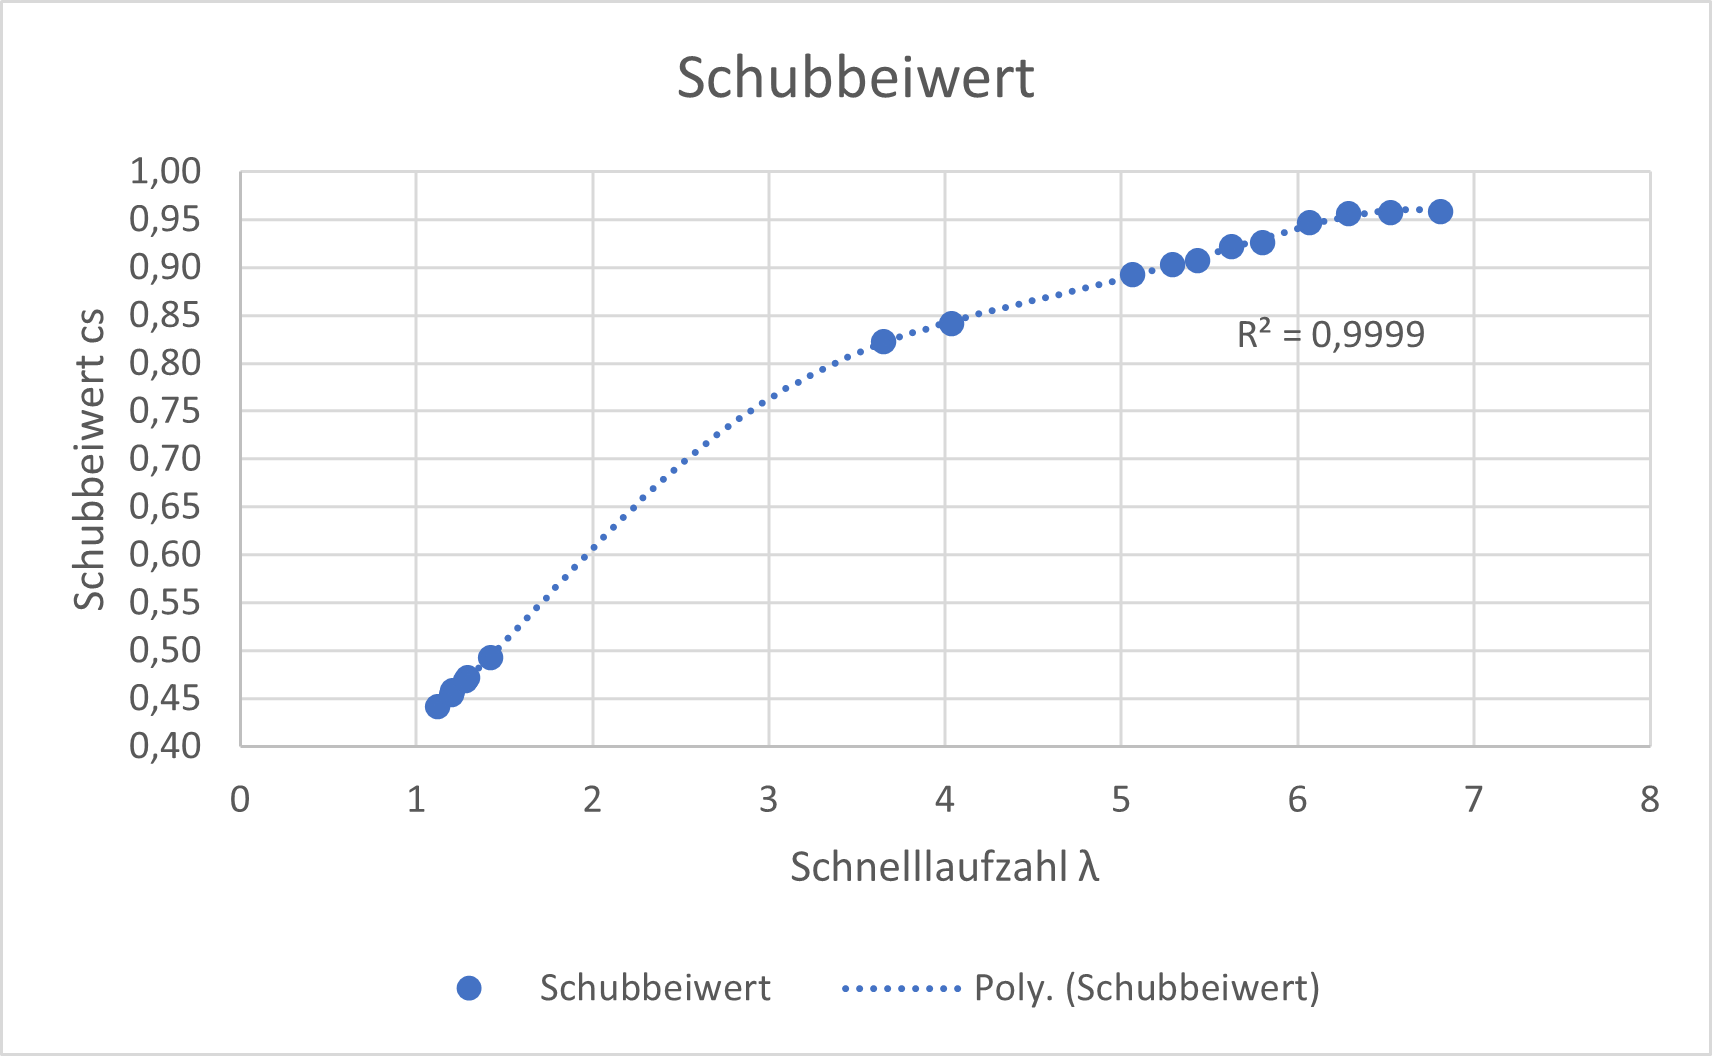
\includegraphics[width=0.9\textwidth]{cs_last}
    \caption{Schubbeiwert $c_s$ in Abhängigkeit von Schnelllaufzahl $\lambda$}
    \label{fig:Schubbeiwert}
\end{figure}

\subsubsection*{Tabelle Messwerte und Dimensionslose Kennzahlen}
\begin{table}[H]
    \centering
    \caption{Dimensionslose Kennzahlen}
    \label{tab:2307028_DimensionsloseKennzahlen}
    \LARGE
    \resizebox{\columnwidth}{!}{%
    \begin{tabular}{|
        >{\columncolor[HTML]{4472C4}}l |
        >{\columncolor[HTML]{4472C4}}l |
        >{\columncolor[HTML]{B4C6E7}}l |
        >{\columncolor[HTML]{D9E1F2}}l |
        >{\columncolor[HTML]{B4C6E7}}l |
        >{\columncolor[HTML]{D9E1F2}}l |
        >{\columncolor[HTML]{B4C6E7}}l |
        >{\columncolor[HTML]{D9E1F2}}l |
        >{\columncolor[HTML]{B4C6E7}}l |
        >{\columncolor[HTML]{D9E1F2}}l |
        >{\columncolor[HTML]{B4C6E7}}l |
        >{\columncolor[HTML]{D9E1F2}}l |
        >{\columncolor[HTML]{B4C6E7}}l |
        >{\columncolor[HTML]{D9E1F2}}l |
        >{\columncolor[HTML]{B4C6E7}}l |
        >{\columncolor[HTML]{D9E1F2}}l |
        >{\columncolor[HTML]{B4C6E7}}l |
        >{\columncolor[HTML]{D9E1F2}}l |
        >{\columncolor[HTML]{B4C6E7}}l |}
        \hline
        \cellcolor[HTML]{70AD47}{\color[HTML]{FFFFFF} \textbf{Schnelllaufzahl}}      & \cellcolor[HTML]{70AD47}-        & \cellcolor[HTML]{C6E0B4}6      & \cellcolor[HTML]{E2EFDA}6      & \cellcolor[HTML]{C6E0B4}6      & \cellcolor[HTML]{E2EFDA}6      & \cellcolor[HTML]{C6E0B4}6      & \cellcolor[HTML]{E2EFDA}6      & \cellcolor[HTML]{C6E0B4}6      & \cellcolor[HTML]{E2EFDA}6      & \cellcolor[HTML]{C6E0B4}6      & \cellcolor[HTML]{E2EFDA}6     & \cellcolor[HTML]{C6E0B4}6      & \cellcolor[HTML]{E2EFDA}6      & \cellcolor[HTML]{C6E0B4}6      & \cellcolor[HTML]{E2EFDA}6      & \cellcolor[HTML]{C6E0B4}6      & \cellcolor[HTML]{E2EFDA}6      & \cellcolor[HTML]{C6E0B4}6      \\ \hline
        \cellcolor[HTML]{70AD47}{\color[HTML]{FFFFFF} \textbf{Pitch}}                & \cellcolor[HTML]{70AD47}in °     & \cellcolor[HTML]{C6E0B4}10     & \cellcolor[HTML]{E2EFDA}10     & \cellcolor[HTML]{C6E0B4}10     & \cellcolor[HTML]{E2EFDA}10     & \cellcolor[HTML]{C6E0B4}10     & \cellcolor[HTML]{E2EFDA}10     & \cellcolor[HTML]{C6E0B4}10     & \cellcolor[HTML]{E2EFDA}10     & \cellcolor[HTML]{C6E0B4}10     & \cellcolor[HTML]{E2EFDA}10    & \cellcolor[HTML]{C6E0B4}10     & \cellcolor[HTML]{E2EFDA}10     & \cellcolor[HTML]{C6E0B4}10     & \cellcolor[HTML]{E2EFDA}10     & \cellcolor[HTML]{C6E0B4}10     & \cellcolor[HTML]{E2EFDA}10     & \cellcolor[HTML]{C6E0B4}10     \\ \hline
        \cellcolor[HTML]{70AD47}{\color[HTML]{FFFFFF} \textbf{Windgeschw.}}          & \cellcolor[HTML]{70AD47}in m/s   & \cellcolor[HTML]{C6E0B4}6,5    & \cellcolor[HTML]{E2EFDA}6,5    & \cellcolor[HTML]{C6E0B4}6,5    & \cellcolor[HTML]{E2EFDA}6,5    & \cellcolor[HTML]{C6E0B4}6,5    & \cellcolor[HTML]{E2EFDA}6,5    & \cellcolor[HTML]{C6E0B4}6,5    & \cellcolor[HTML]{E2EFDA}6,5    & \cellcolor[HTML]{C6E0B4}6,5    & \cellcolor[HTML]{E2EFDA}6,5   & \cellcolor[HTML]{C6E0B4}6,5    & \cellcolor[HTML]{E2EFDA}6,5    & \cellcolor[HTML]{C6E0B4}6,5    & \cellcolor[HTML]{E2EFDA}6,5    & \cellcolor[HTML]{C6E0B4}6,5    & \cellcolor[HTML]{E2EFDA}6,5    & \cellcolor[HTML]{C6E0B4}6,5    \\ \hline
        \cellcolor[HTML]{5B9BD5}{\color[HTML]{FFFFFF} \textbf{v1 Mittelwert}}        & \cellcolor[HTML]{5B9BD5}m/s      & \cellcolor[HTML]{BDD7EE}6,48   & \cellcolor[HTML]{DDEBF7}6,47   & \cellcolor[HTML]{BDD7EE}6,45   & \cellcolor[HTML]{DDEBF7}6,44   & \cellcolor[HTML]{BDD7EE}6,41   & \cellcolor[HTML]{DDEBF7}6,44   & \cellcolor[HTML]{BDD7EE}6,41   & \cellcolor[HTML]{DDEBF7}6,42   & \cellcolor[HTML]{BDD7EE}6,39   & \cellcolor[HTML]{DDEBF7}6,41  & \cellcolor[HTML]{BDD7EE}6,43   & \cellcolor[HTML]{DDEBF7}6,38   & \cellcolor[HTML]{BDD7EE}6,39   & \cellcolor[HTML]{DDEBF7}6,44   & \cellcolor[HTML]{BDD7EE}6,39   & \cellcolor[HTML]{DDEBF7}6,42   & \cellcolor[HTML]{BDD7EE}6,42   \\ \hline
        \cellcolor[HTML]{5B9BD5}{\color[HTML]{FFFFFF} \textbf{Turbulenz}}            & \cellcolor[HTML]{5B9BD5}m/s      & \cellcolor[HTML]{BDD7EE}0,0185 & \cellcolor[HTML]{DDEBF7}0,0303 & \cellcolor[HTML]{BDD7EE}0,0212 & \cellcolor[HTML]{DDEBF7}0,0134 & \cellcolor[HTML]{BDD7EE}0,0174 & \cellcolor[HTML]{DDEBF7}0,0238 & \cellcolor[HTML]{BDD7EE}0,0209 & \cellcolor[HTML]{DDEBF7}0,0228 & \cellcolor[HTML]{BDD7EE}0,0175 & \cellcolor[HTML]{DDEBF7}0,024 & \cellcolor[HTML]{BDD7EE}0,0246 & \cellcolor[HTML]{DDEBF7}0,0299 & \cellcolor[HTML]{BDD7EE}0,1889 & \cellcolor[HTML]{DDEBF7}0,0293 & \cellcolor[HTML]{BDD7EE}0,0192 & \cellcolor[HTML]{DDEBF7}0,0237 & \cellcolor[HTML]{BDD7EE}0,2556 \\ \hline
        \cellcolor[HTML]{5B9BD5}{\color[HTML]{FFFFFF} \textbf{V3 Mittelwert}}        & \cellcolor[HTML]{5B9BD5}m/s      & \cellcolor[HTML]{BDD7EE}3,53   & \cellcolor[HTML]{DDEBF7}3,456  & \cellcolor[HTML]{BDD7EE}3,495  & \cellcolor[HTML]{DDEBF7}3,289  & \cellcolor[HTML]{BDD7EE}3,21   & \cellcolor[HTML]{DDEBF7}3,147  & \cellcolor[HTML]{BDD7EE}3,116  & \cellcolor[HTML]{DDEBF7}3,189  & \cellcolor[HTML]{BDD7EE}2,963  & \cellcolor[HTML]{DDEBF7}2,992 & \cellcolor[HTML]{BDD7EE}3,128  & \cellcolor[HTML]{DDEBF7}4,498  & \cellcolor[HTML]{BDD7EE}4,407  & \cellcolor[HTML]{DDEBF7}4,486  & \cellcolor[HTML]{BDD7EE}4,511  & \cellcolor[HTML]{DDEBF7}4,389  & \cellcolor[HTML]{BDD7EE}4,321  \\ \hline
        {\color[HTML]{FFFFFF} \textbf{v3/v1}}                                        & -                                & 0,545                          & 0,534                          & 0,542                          & 0,511                          & 0,501                          & 0,489                          & 0,486                          & 0,496                          & 0,464                          & 0,467                         & 0,487                          & 0,706                          & 0,689                          & 0,697                          & 0,706                          & 0,684                          & 0,673                          \\ \hline
        {\color[HTML]{FFFFFF} \textbf{Windleistung}}                                 & W                                & 14,809                         & 14,734                         & 14,631                         & 14,557                         & 14,341                         & 14,563                         & 14,347                         & 14,442                         & 14,194                         & 14,321                        & 14,455                         & 14,114                         & 14,234                         & 14,536                         & 14,227                         & 14,388                         & 14,401                         \\ \hline
        \cellcolor[HTML]{70AD47}{\color[HTML]{FFFFFF} \textbf{Last}}                 & \cellcolor[HTML]{70AD47}in \%    & \cellcolor[HTML]{C6E0B4}0      & \cellcolor[HTML]{E2EFDA}5      & \cellcolor[HTML]{C6E0B4}10     & \cellcolor[HTML]{E2EFDA}15     & \cellcolor[HTML]{C6E0B4}20     & \cellcolor[HTML]{E2EFDA}25     & \cellcolor[HTML]{C6E0B4}30     & \cellcolor[HTML]{E2EFDA}35     & \cellcolor[HTML]{C6E0B4}40     & \cellcolor[HTML]{E2EFDA}45    & \cellcolor[HTML]{C6E0B4}50     & \cellcolor[HTML]{E2EFDA}55     & \cellcolor[HTML]{C6E0B4}60     & \cellcolor[HTML]{E2EFDA}65     & \cellcolor[HTML]{C6E0B4}70     & \cellcolor[HTML]{E2EFDA}75     & \cellcolor[HTML]{C6E0B4}80     \\ \hline
        \cellcolor[HTML]{5B9BD5}{\color[HTML]{FFFFFF} \textbf{Rotordrehzahl}}        & \cellcolor[HTML]{5B9BD5}in min-1 & 2478,8                         & 2371,1                         & 2279,4                         & 2196,2                         & 2089,2                         & 2035,8                         & 1956,5                         & 1908,4                         & 1817,1                         & 1452,9                        & 1318,4                         & 402,1                          & 462,8                          & 435,4                          & 431,4                          & 460,8                          & 511,6                          \\ \hline
        {\color[HTML]{FFFFFF} \textbf{Umfangsgeschw.}}                               & m/s                              & 44,128                         & 42,211                         & 40,579                         & 39,098                         & 37,193                         & 36,242                         & 34,830                         & 33,974                         & 32,349                         & 25,865                        & 23,471                         & 7,158                          & 8,239                          & 7,751                          & 7,680                          & 8,203                          & 9,108                          \\ \hline
        {\color[HTML]{FFFFFF} \textbf{Schnellaufzahl}}                               & -                                & 6,812                          & 6,527                          & 6,289                          & 6,070                          & 5,803                          & 5,626                          & 5,434                          & 5,289                          & 5,065                          & 4,038                         & 3,652                          & 1,123                          & 1,289                          & 1,204                          & 1,201                          & 1,279                          & 1,419                          \\ \hline
        \cellcolor[HTML]{5B9BD5}{\color[HTML]{FFFFFF} \textbf{Drehmoment Rotor}}     & \cellcolor[HTML]{5B9BD5}in mNm   & 11,0                           & 17,0                           & 22,4                           & 26,6                           & 31,1                           & 35,1                           & 38,6                           & 42,3                           & 46,9                           & 68,2                          & 76,5                           & 46,4                           & 51,4                           & 49,5                           & 48,6                           & 51,8                           & 55,1                           \\ \hline
        {\color[HTML]{FFFFFF} \textbf{Drehmoment Generator}}                         & mNm                              & 4,70                           & \cellcolor[HTML]{B4C6E7}10,74  & 16,11                          & \cellcolor[HTML]{B4C6E7}20,29  & 24,79                          & \cellcolor[HTML]{B4C6E7}28,83  & 32,34                          & \cellcolor[HTML]{B4C6E7}36,01  & 40,60                          & \cellcolor[HTML]{B4C6E7}61,87 & 70,25                          & \cellcolor[HTML]{B4C6E7}40,10  & 45,12                          & \cellcolor[HTML]{B4C6E7}43,24  & 42,26                          & \cellcolor[HTML]{B4C6E7}45,46  & 48,85                          \\ \hline
        {\color[HTML]{FFFFFF} \textbf{Mechanische Leistung}}                         & W                                & 1,22                           & 2,67                           & 3,85                           & 4,67                           & 5,42                           & 6,15                           & 6,63                           & 7,20                           & 7,73                           & 9,41                          & 9,70                           & 1,69                           & 2,19                           & 1,97                           & 1,91                           & 2,19                           & 2,62                           \\ \hline
        {\color[HTML]{FFFFFF} \textbf{Momentbeiwert}}                                & -                                & 0,012                          & 0,028                          & 0,042                          & 0,053                          & 0,065                          & 0,075                          & 0,085                          & 0,094                          & 0,107                          & 0,163                         & 0,184                          & 0,107                          & 0,119                          & 0,113                          & 0,112                          & 0,119                          & 0,128                          \\ \hline
        \cellcolor[HTML]{5B9BD5}{\color[HTML]{FFFFFF} \textbf{Generatorspannung}}    & \cellcolor[HTML]{5B9BD5}in V     & 9,8                            & 9,0                            & 8,5                            & 7,9                            & 7,6                            & 6,8                            & 6,4                            & 6,5                            & 6,1                            & 3,9                           & 3,0                            & 0,2                            & 0,3                            & 0,3                            & 0,2                            & 0,3                            & 0,3                            \\ \hline
        \cellcolor[HTML]{5B9BD5}{\color[HTML]{FFFFFF} \textbf{Generatorstrom}}       & \cellcolor[HTML]{5B9BD5}in A     & 0,0                            & 0,1                            & 0,2                            & 0,2                            & 0,3                            & 0,3                            & 0,4                            & 0,4                            & 0,5                            & 0,8                           & 0,9                            & 0,5                            & 0,6                            & 0,5                            & 0,6                            & 0,6                            & 0,6                            \\ \hline
        {\color[HTML]{FFFFFF} \textbf{Elektrische Leistung}}                         & W                                & 0,210                          & 0,990                          & 1,479                          & 1,841                          & 2,212                          & 2,315                          & 2,477                          & 2,875                          & 3,117                          & 3,120                         & 2,745                          & 0,131                          & 0,165                          & 0,142                          & 0,150                          & 0,160                          & 0,185                          \\ \hline
        {\color[HTML]{FFFFFF} \textbf{Elektrischer Leistungsbeiwert}}                & -                                & 1,42\%                         & 6,72\%                         & 10,11\%                        & 12,65\%                        & 15,42\%                        & 15,90\%                        & 17,26\%                        & 19,91\%                        & 21,96\%                        & 21,79\%                       & 18,99\%                        & 0,93\%                         & 1,16\%                         & 0,97\%                         & 1,05\%                         & 1,11\%                         & 1,28\%                         \\ \hline
        {\color[HTML]{FFFFFF} \textbf{Leistungsbeiwert}}                             & -                                & 0,082                          & 0,181                          & 0,263                          & 0,321                          & 0,378                          & 0,422                          & 0,462                          & 0,498                          & 0,544                          & 0,657                         & 0,671                          & 0,120                          & 0,154                          & 0,136                          & 0,134                          & 0,152                          & 0,182                          \\ \hline
        {\color[HTML]{FFFFFF} \textbf{Generator Wirkungsgrad}}                       & -                                & 17,19\%                        & 37,14\%                        & 38,45\%                        & 39,44\%                        & 40,77\%                        & 37,68\%                        & 37,38\%                        & 39,95\%                        & 40,35\%                        & 33,14\%                       & 28,30\%                        & 7,75\%                         & 7,55\%                         & 7,19\%                         & 7,84\%                         & 7,27\%                         & 7,05\%                         \\ \hline
        \cellcolor[HTML]{5B9BD5}{\color[HTML]{FFFFFF} \textbf{Normalkraft}}          & \cellcolor[HTML]{5B9BD5}N        & \cellcolor[HTML]{BDD7EE}1,048  & \cellcolor[HTML]{DDEBF7}1,043  & \cellcolor[HTML]{BDD7EE}1,037  & \cellcolor[HTML]{DDEBF7}1,024  & \cellcolor[HTML]{BDD7EE}0,991  & \cellcolor[HTML]{DDEBF7}0,997  & \cellcolor[HTML]{BDD7EE}0,972  & \cellcolor[HTML]{DDEBF7}0,971  & \cellcolor[HTML]{BDD7EE}0,949  & \cellcolor[HTML]{DDEBF7}0,900 & \cellcolor[HTML]{BDD7EE}0,885  & \cellcolor[HTML]{DDEBF7}0,468  & \cellcolor[HTML]{BDD7EE}0,503  & \cellcolor[HTML]{DDEBF7}0,495  & \cellcolor[HTML]{BDD7EE}0,484  & \cellcolor[HTML]{BDD7EE}0,503  & \cellcolor[HTML]{BDD7EE}0,529  \\ \hline
        \cellcolor[HTML]{5B9BD5}{\color[HTML]{FFFFFF} \textbf{Schubkraft auf Rotor}} & \cellcolor[HTML]{5B9BD5}N        & \cellcolor[HTML]{BDD7EE}2,191  & \cellcolor[HTML]{DDEBF7}2,180  & \cellcolor[HTML]{BDD7EE}2,168  & \cellcolor[HTML]{DDEBF7}2,140  & \cellcolor[HTML]{BDD7EE}2,072  & \cellcolor[HTML]{DDEBF7}2,083  & \cellcolor[HTML]{BDD7EE}2,030  & \cellcolor[HTML]{DDEBF7}2,030  & \cellcolor[HTML]{BDD7EE}1,984  & \cellcolor[HTML]{DDEBF7}1,882 & \cellcolor[HTML]{BDD7EE}1,850  & \cellcolor[HTML]{DDEBF7}0,977  & \cellcolor[HTML]{BDD7EE}1,051  & \cellcolor[HTML]{DDEBF7}1,035  & \cellcolor[HTML]{BDD7EE}1,011  & \cellcolor[HTML]{BDD7EE}1,051  & \cellcolor[HTML]{BDD7EE}1,105  \\ \hline
        {\color[HTML]{FFFFFF} \textbf{Schubbeiwert}}                                 &                                  & 0,958                          & 0,957                          & 0,956                          & 0,947                          & 0,926                          & 0,921                          & 0,907                          & 0,903                          & 0,893                          & 0,842                         & 0,823                          & 0,442                          & 0,472                          & 0,458                          & 0,454                          & \cellcolor[HTML]{B4C6E7}0,469  & 0,492                          \\ \hline
        {\color[HTML]{FFFFFF} \textbf{R\_Last}}                                      &                                  & 457,944                        & 81,818                         & 48,286                         & 33,906                         & 26,117                         & 19,679                         & 16,282                         & 14,650                         & 11,937                         & 4,875                         & 3,279                          & 0,470                          & 0,458                          & 0,477                          & 0,401                          & \cellcolor[HTML]{B4C6E7}0,474  & 0,488                          \\ \hline
        \end{tabular}%
    }
    \end{table}

\subsection{Feedback zum Versuch}

Der Versuch vermittelt ein gutes Verständnis über die Notwendigkeit und den Gebrauch des Pitchwinkels. Allerdings wäre eine Überarbeitung des Programms, welche die Messdaten aufnimmt 
empfehlenswert, da diese sehr schwer nachzuvollziehen sind. Auch eine genauere Erklärung zu dem Programm, den Messdaten und den Einheiten, in welche die Daten aufgenommen werden, könnte in der Versuchsanleitung hilfreich sein.
(Zu viel Kritik? lieber weg lassen?)